\chapter{Construcción del sistema}
\label{chap:SystemConstruction}

En este capítulo serán presentados los subsistemas que fueron desarrollados, siguiendo los lineamientos presentados en el capítulo de arquitectura (publicada como artículo independiente en \textcolor{red}{Autocita}), de forma que se vea la construcción a partir de las diferentes plantillas (\ref{Sec:DeviceControllerTemplate}, \ref{Sec:ClassifierHARTemplate}, \ref{Sec:EventAnalyzerTemplate}, \ref{Sec:NotifierChannelTemplate}). De igual forma que la arquitectura, algunos de los submódulos, por su propia naturaleza e impacto en el campo de reconocimiento de actividad humana, dieron origen a artículos específicos.

\selectlanguage{english} % Selección de idioma del resumen.
\textbf{Scalable architecture for the integration of multiple AI systems applied to smart environments (Abstract)}
\begin{quote}
Currently, one of the most relevant topics in research is the use of artificial intelligence (AI) algorithms in different areas. Within the wide range of algorithms, the use of artificial neural networks (ANN) stands out.In the ANN there are different designs, with different inputs and outputs, each adjusted to the needs of the problem they solve. However, it is not always easy to integrate the results from one to another, for example, if we have a system that must act according to three questions: are there people in an image?, what command did a person say?, is there enough milk for tomorrow's breakfast?, so the system must be constructed to process the three questions simultaneously, in this way, each question can be answered by a different ANN or even by another AI technique, generating different forms of answers. The system designer could solve this problem in two ways, first, by designing a very large ANN with a very high number of inputs, outputs and hidden layers to receive all possible forms of input and output. This could be easy in this case but, if the number of questions is very large or even unknown from the beginning, this task could be more complicated or non-viable, limiting size of the system. The second option is to keep ANN separate for each question and design a specific subsystem to join all the results, this option is more flexible but could affect performance if the distributed processing is not consider. In this paper we present an architecture that allows many artificial intelligence systems to be integrated, regardless of technique, algorithm, data source or even system output, without affecting performance because it allows highly distributed execution and robust enough to shut down or add subsystems without affecting the others.
\end{quote}
\selectlanguage{spanish} % Selección de idioma del resumen.
\textbf{Arquitectura escalable para la integración de múltiples sistemas de IA aplicados a entornos inteligentes. (Resumen)}
\begin{quote}
Actualmente, uno de los temas más relevantes en la investigación es el uso de algoritmos de inteligencia artificial (IA) en diferentes áreas. Dentro de la amplia gama de algoritmos, destaca el uso de redes neuronales artificiales (ANN). En el ANN hay diferentes diseños, con diferentes entradas y salidas, cada uno ajustado a las necesidades del problema que resuelven. Sin embargo, no siempre es fácil integrar los resultados de uno a otro, por ejemplo, si tenemos un sistema que debe actuar de acuerdo con tres preguntas: ¿hay personas en una imagen?, ¿qué comando dijo una persona? ¿suficiente leche para el desayuno de mañana?, entonces el sistema debe ser construido para procesar las tres preguntas simultáneamente, de esta manera, cada pregunta puede ser respondida por un ANN diferente o incluso por otra técnica de IA, generando diferentes formas de respuestas. El diseñador del sistema podría resolver este problema de dos maneras, primero, diseñando un ANN muy grande con un número muy alto de entradas, salidas y capas ocultas para recibir todas las formas posibles de entrada y salida. Esto podría ser fácil en este caso pero, si el número de preguntas es muy grande o incluso desconocido desde el principio, esta tarea podría ser más complicada o no viable, limitando el tamaño del sistema. La segunda opción es mantener a ANN separada para cada pregunta y diseñar un subsistema específico para unir todos los resultados, esta opción es más flexible pero podría afectar el rendimiento si no se considera el procesamiento distribuido. En este artículo presentamos una arquitectura que permite la integración de muchos sistemas de inteligencia artificial, independientemente de la técnica, el algoritmo, la fuente de datos o incluso la salida del sistema, sin afectar el rendimiento porque permite una ejecución altamente distribuida y lo suficientemente robusta para apagar o agregar subsistemas sin afectar los demás.
\end{quote}
\newpage

\section{Módulo para incluir las cámaras web como un tipo sensor del sistema}
    Parte fundamental de cualquier sistema es la entrada de datos, para este sistema se ha creado un componente extensible llamado ``DeviceController'' (Ver sección \ref{sub:DeviceController}). Este componente contienen los métodos y atributos necesarios para transformar los datos capturados de un dispositivo especifico y enviarlos a la pila de datos. Sin embargo, para la utilización de los distintos dispositivos físicos de que se dispongan, será necesario la creación de una clase especifica que extiende a ``DeviceController'', como se ve en la figura \ref{fig:CamControllerClassModel}, y contiene la lógica que permite leer el dispositivo.
    
    \begin{figure}[ht!]
    	\centering
    	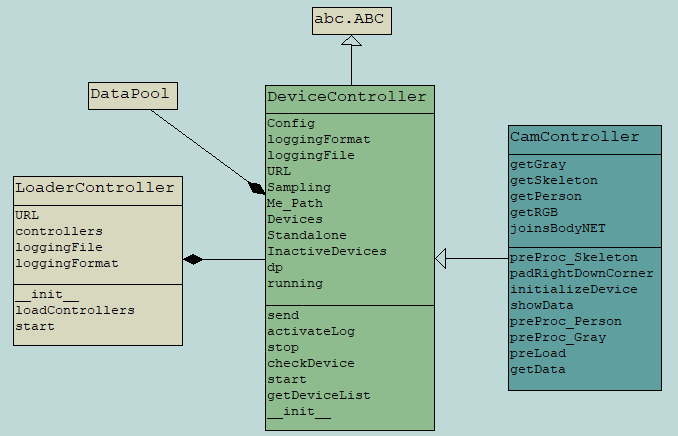
\includegraphics[width=0.9\linewidth]{imgs/04-Construction/04-ControllerClassModel.PNG}
    	\caption[Modelo de clases de CamController]{Modelo de clases de CamController. Presenta las la relación y dependencias de las clases del controlador de cámaras.}
	    \label{fig:CamControllerClassModel}
    \end{figure}%
    
    Siguiendo las instrucciones descritas en la sección \ref{Sec:DeviceControllerTemplate}, para este proyecto se estableció la captura de imágenes por medio de cámaras RGB tradicionales, por ser éstas un dispositivo de fácil adquisición y bajo coste, lo que permite la utilización de varias cámaras en un hogar, objeto fundamental de este trabajo. Sin embargo, se reitera que el diseño de este sistema no se limita a aun tipo de dispositivo.
    
    El controlador de cámaras consta principalmente de cuatro archivos: 
    \begin{itemize}
        \item config.yaml
        \item devices.yaml
        \item CamController.py
        \item model/poseModel.h5
    \end{itemize}
    
    El archivo \textbf{config.yaml} además de las variables mencionadas en la sección \ref{sub2:ConfigFileController} contiene algunas de uso específico en este controlador (ver tabla \ref{Tab:ConfigFileCamController}).
    
    \begin{table}[ht!]
    \caption[Archivo de configuración de CamController]{Atributos del archivo de configuración de CamController.}
    \label{Tab:ConfigFileCamController}
    \centering
    \begin{tabular}{ | l l p{6cm} | } 
        \hline
        \textbf{Atributo}       & \textbf{Valor} & \textbf{Descripción} \\ 
        \hline\hline
        \textbf{FRAME\_WIDTH}   & 320 & Ancho de la imagen capturada.\\
        \hline
        \textbf{FRAME\_HEIGHT}  & 240 & Alto de la imagen capturada.\\
        \hline
        \textbf{FORMATS}        & [RGB, Gray, Objects] & transformaciónes que se aplicaran a los datos capturados. Pueden ser combinados para retornar uno o varios. los valores disponibles son: RGB, Gray, Person, Skeleton.\\
        \hline
        \textbf{OBJECTS}        & [Person,] & Listado de 80 posibles objetos detectables. Esto se apoya en el trabajo Mask-RCNN (He et al. en \cite{He2017}). \\
        \hline
    \end{tabular}
    \end{table}
    
    El archivo \textbf{devices.yaml} contiene el listado de cámaras que serán utilizadas, pudiendo identificar cada una con una etiqueta. El fragmento de código alg. \ref{Alg:devicesCamController} presenta la estructura del archivo. En este caso las configuraciones se aplicaran a cada cámara por separado, siendo posible activar o desactivar una cámara o cambiar el ancho y alto de la imagen capturada.
    
    \lstinputlisting[language=Python, caption={Cámaras disponibles.}, label=Alg:devicesCamController]{code/04-Construction/04-devices.yaml}

    El archivo \textbf{CamController.py} contiene toda la lógica que permite funcionar al componente. Dentro de este archivo se encuentra una clase que lleva el mismo nombre y hereda de ``DeviceController''. Esta clase implementa, en primera instancia, los métodos abstractos de la clase padre. Además, contiene los métodos que permiten hacer las transformaciones a los datos originales como muestra la tabla \ref{Tab:CamControllerOwnMethods}.
    
    \begin{table}[ht!]
    \caption[Archivo de configuración de CamController]{Atributos del archivo de configuración de CamController.}
    \label{Tab:CamControllerOwnMethods}
    \centering
    \begin{tabular}{ | l p{8cm} | } 
        \hline
        \textbf{Método}         & \textbf{Descripción} \\ 
        \hline\hline
        \textbf{preProc\_Gray}     & Convierte la imagen a escala de grises suando la formula Y = 0.299 * R + 0.587 * G + 0.114 * B.\\
        \hline
        \textbf{preProc\_Object}   & Procesa la imagen capturada y retorna una lista de imágenes que contiene de forma separado cada objeto detectado, extraído del fondo.\\
        \hline
        \textbf{preProc\_Skeleton} & Procesa la imagen capturada y retorna una lista de puntos con las coordenadas de las articulaciones de las personas en la imágen.\\
        \hline
        \textbf{"\_\_main\_\_"}    & Permite la ejecución del componente de forma independiente al sistema, de esta forma poder visualizar directamente los datos que se están capturando y las transformaciones realizadas.\\
        \hline
    \end{tabular}
    \end{table}
    
    \begin{figure}[ht!]
    	\centering
    	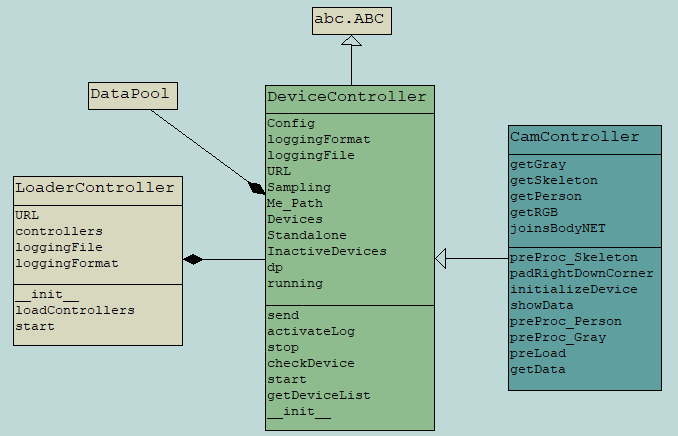
\includegraphics[width=0.9\linewidth]{imgs/04-Construction/04-ControllerClassModel.PNG}
    	\caption[Captura y transformaciones del CamController]{Captura y transformaciones del CamController. a) RGB, b) Grises, c) Persona extraída, d) Esqueleto. \textcolor{red}{Cambio de imagen, RGB Gray, PErson y Skeleton}}
    	
	    \label{fig:CamControllerTransGetData}
    \end{figure}%
    
    \subsection{Extracción de la persona}
    \label{Sub:MakePerson}
         Para localizar y extraer las personas registradas en las imágenes se utilizó el trabajo presentado por He et al. en \cite{He2017}, ya que éste permite la la detección de las personas y retorna la mascara o conjunto de píxeles que la componen, simplificando el proceso de extraer y recortar la imagen, para así retornar una nube de puntos por cada persona detectada. Adicionalmente, el trabajo de He permite la extracción de 80 objetos adicionales, lo cual podría permitir a futuro la ampliación de este componente.
        
    \subsection{Extracción del esqueleto}
    \label{Sub:MakeSkeleton}
        La esqueletonización consiste en la extracción de los puntos del cuerpo de una persona que permiten reconstruir una versión simplificada de la postura de la persona. Como se menciono en la sección \ref{sub:FramePoseEstimation} existen diferentes estrategias para lograrlo. En este proceso se basa en el trabajo de Cao et al. \cite{Cao2017}, que usa el concepto de mapas de calor para estimar zonas candidatas donde es posible encontrar una articulación de una personas, logrando generar hasta un total de 18 puntos por cada persona localizada.
        
\section{Construcción de módulo para el reconocimiento de infartos}
\label{Sec:InfarctDetectModule}

    Esta sección describe la utilización de la plantilla diseñada para la creación de módulos para el reconocimiento de actividades humanas (HAR\index{HAR}). Para ello se definió un evento específico que puede ocurrir a cualquier persona. Las enfermedades cardiovasculares, según estudios de la Organización Mundial de la Salud (OMS), una de las principales causas de muerte en el mundo \cite{OMS2018}. Adicionalmente, cuando una persona sufre un ataque al corazón, experimenta un fuerte dolor en el pecho \cite{Patel2018, Goff1998}, que puede conducir a la pérdida de la conciencia y de encontrarse solo o sola no recibir ayuda oportuna. 
    
    \subsection{Detección de ataque cardíaco en imágenes en color utilizando redes neuronales convolucionales}
    \label{sub:InfarctColorMethod}
    
        El desarrollo de este módulo dio como resultado la publicación 'Heart Attack Detection in Colour Images Using Convolutional Neural Networks' \cite{rojas2019heart}. El código asociado a este artículo puede ser descargado de forma independiente de \url{https://github.com/Turing-IA-IHC/Heart-Attack-Detection-In-Images}.
        
        \selectlanguage{english} % Selección de idioma del resumen.
        \textbf{Heart Attack Detection in Colour Images Using Convolutional Neural Networks (Abstract)}
        \begin{quote}
        Cardiovascular diseases are the leading cause of death worldwide. Therefore, getting help in time makes the difference between life and death. In many cases, help is not obtained in time when a person is alone and suffers a heart attack. This is mainly due to the fact that pain prevents him/her from asking for help. This article presents a novel proposal to identify people with an apparent heart attack in colour images by detecting characteristic postures of heart attack. The method identifying infarcts makes use of convolutional neural networks. These have been trained with a specially prepared set of images that contain people simulating a heart attack. The promising results in the classification of infarcts show 91.75\% accuracy and 92.85\% sensitivity.
        \end{quote}
        \selectlanguage{spanish} % Selección de idioma del resumen.
        \textbf{Detección de ataque cardíaco en imágenes en color utilizando redes neuronales convolucionales. (Resumen)}
        \begin{quote}
        Las enfermedades cardiovasculares son la principal causa de muerte en todo el mundo. Por lo tanto, obtener ayuda a tiempo marca la diferencia entre la vida y la muerte. En muchos casos, no se obtiene ayuda a tiempo cuando una persona está sola y sufre un ataque cardíaco. Esto se debe principalmente al hecho de que el dolor le impide pedir ayuda. Este artículo presenta una nueva propuesta para identificar a las personas con un aparente ataque al corazón en imágenes en color mediante la detección de posturas características del ataque al corazón. El método para identificar infartos utiliza redes neuronales convolucionales. Estos han sido entrenados con un conjunto de imágenes especialmente preparadas que contienen personas que simulan un ataque cardíaco. Los resultados prometedores en la clasificación de infartos muestran 91.75\% de precisión y 92.85\% de sensibilidad.
        \end{quote}
        
        Siguiendo los lineamientos de arquitectura se generó el módulo de nombre ``ColorInfarctRecognizer'', para la identificación de posibles eventos de infarto.
        
        \begin{figure}[ht!]
        	\centering
        	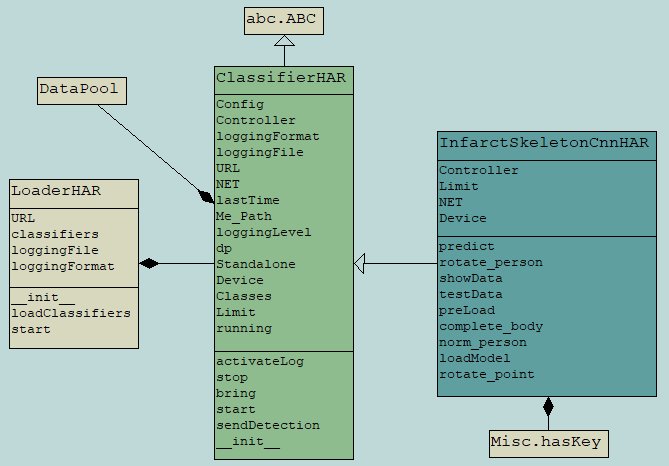
\includegraphics[width=0.9\linewidth]{imgs/04-Construction/04-HarClassModel.PNG}
        	\caption[Modelo de clases de ColorInfarctRecognizer]{Modelo de clases de ColorInfarctRecognizer. Presenta las la relación y dependencias de las clases del módulo para identificación de eventos de posibles infartos de personas.}
    	    \label{fig:InfarctHARClassModel}
        \end{figure}%
        
        El módulo para la identificación de posibles infartos consta de los siguientes archivos:
        
        \begin{itemize}
            \item config.yaml
            \item ColorInfarctRecognizer.py
            \item model/rgbInfarctModel.h5
        \end{itemize}
        
        El archivo \textbf{config.yaml} contiene las variables mencionadas en la sección \ref{sub2:ConfigFileHAR} donde se resalta especialmente las variables de 'FILTER\_NAME' y 'CLASSES' (ver tabla \ref{Tab:ConfigFileInfarctHAR}), siendo el tipo de información a analizar y los eventos a detectar respectivamente.
        
        \begin{table}[ht!]
        \caption[Archivo de configuración de ColorInfarctRecognizer]{Atributos del archivo de configuración de ColorInfarctRecognizer.}
        \label{Tab:ConfigFileInfarctHAR}
        \centering
        \begin{tabular}{ | l l p{6cm} | } 
            \hline
            \textbf{Atributo}       & \textbf{Valor} & \textbf{Descripción} \\ 
            \hline\hline
            \textbf{FILTER\_NAME}   & CamController/person & Imagen de una persona extraída del fondo.\\
            \hline
            \textbf{CLASSES}  & [None, Infarct] & Siendo 'None' una clase genérica para indicar la ausencia de evento detectado e 'Infarct' la identificación de una persona con posible infarto.\\
            \hline
            \textbf{MODEL}        & model/rgbInfarctModel.h5  &  Entrenamiento previo que permite la identificación de las personas con un posible infarto.\\
            \hline
        \end{tabular}
        \end{table}
        
        El archivo \textbf{ColorInfarctRecognizer.py} contiene toda la lógica que permite funcionar al componente. Dentro de este archivo se encuentra una clase que lleva el mismo nombre y hereda de ``ColorInfarctRecognizer''. Esta clase implementa los métodos abstractos de la clase padre, siendo particularmente relevante y exclusivo, respecto a otros componentes, la implementación del método '\textbf{\textit{predict}}'.
        
        \begin{figure}[ht!]
        	\centering
        	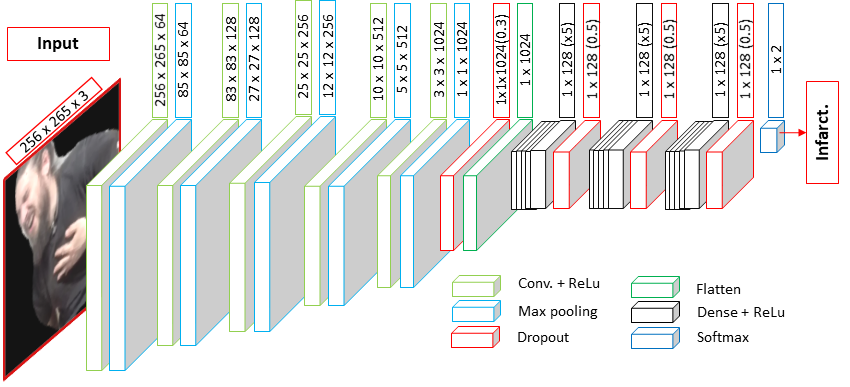
\includegraphics[width=0.9\linewidth]{imgs/04-Construction/04-InfarctBasic-Network.png}
        	\caption[Red neuronal usada por ColorInfarctRecognizer]{Red neuronal usada por ColorInfarctRecognizer. Presenta las capas que definen la red para la inderencia de infartos en imágenes RGB tradicionales.}
    	    \label{fig:InfarctBasic-Network}
        \end{figure}%
        
        El método '\textbf{\textit{predict}}', ejecuta la predicción de si una persona puede estar teniendo un infarto, usando una imagen de la que se ha extraído una persona del fondo, esto es cambiar cualquier píxel del fondo por un color único (morado). La imagen es pasada a la red neuronal previamente entrenada, la cual tiene dos salidas, si el porcentaje de la segunda es mayor que la primera, entonces se entenderá como 'infarto' (ver figura \ref{Alg:ColorInfarctRecognizerPredict}). Además, para cumplir con los requisitos de ingreso de los datos a la red neuronal, este método ajusta el tamaño de la imagen para escalarla a 256x256 píxeles (ver alg. \ref{Alg:ColorInfarctRecognizerPredict}).
                
        \lstinputlisting[language=Python, caption={Predicción de infarto del módulo ColorInfarctRecognizer.}, label=Alg:ColorInfarctRecognizerPredict]{code/03-Architecture/ColorInfarctRecognizer-predict.py}
    
    \subsection{Use of skeletons and facial expressions to identify heart attacks}
    \label{sub:InfarctSkeletonMethod}
        Tomando un enfoque diferente para la identificación de posibles infartos en humanos, se propuso un nuevo componente, con una una estrategia diferentes con el objetivo adicional de reducir los tiempos de procesamiento requeridos manteniendo la precisión. En este caso en lugar de analizar toda la persona solo se considero los puntos que forman el esqueleto y la expresión del rostro (ver figura \ref{fig:Skeleton-FullProcess}), dando como resultado el artículo \textcolor{red}{Cita a Use of skeletons and facial expressions}.
        
        \selectlanguage{english} % Selección de idioma del resumen.
        \textbf{Use of pose estimation and pain face identification to identify heart attacks in images (Abstract)}
        \begin{quote}
        Many cases in which deaths occur due to heart attacks, the person was alone. Getting help quickly makes the difference between life and death, however, felt pain can prevent the person from asking for help. For this reason, it is appropriate to have a mechanism that identifies these events automatically. In this article we present a work developed in this line, in the first instance we show two ways to identify the posture using the upper joints of the body. In addition to this, it is understandable that a person can have similar positions without suffering a heart attack, which leads to a high number of false positives, to reduce this we perform additional processing to verify that, in addition to the posture, the person shows a expression of pain on his or her face.
        \end{quote}
        \selectlanguage{spanish} % Selección de idioma del resumen.
        \textbf{Uso de la estimación de pose y la identificación de la cara del dolor para identificar ataques cardíacos en imágenes. (Resumen)}
        \begin{quote}
        Muchos casos en los que ocurren muertes debido a ataques cardíacos, la persona estaba sola. Obtener ayuda rápidamente hace la diferencia entre la vida y la muerte, sin embargo, sentir dolor puede evitar que la persona pida ayuda. Por esta razón, es apropiado tener un mecanismo que identifique estos eventos automáticamente. En este artículo presentamos un trabajo desarrollado en esta línea, en primera instancia mostramos dos formas de identificar la postura utilizando las articulaciones superiores del cuerpo. Además de esto, es comprensible que una persona pueda tener posiciones similares sin sufrir un ataque cardíaco, lo que conduce a una gran cantidad de falsos positivos, para reducir esto realizamos un procesamiento adicional para verificar que, además de la postura, la persona muestra una expresión de dolor en su rostro.
        \end{quote}
        
        \begin{figure}[ht!]
        	\centering
        	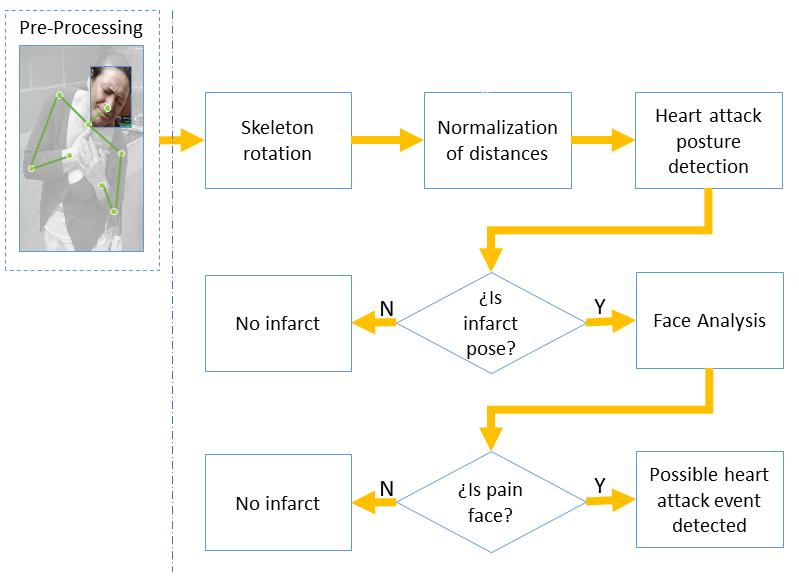
\includegraphics[width=0.9\linewidth]{imgs/04-Construction/04-Skeleton-FullProcess.png}
        	\caption[Flujo de reconocimiento de infartos del módulo SkeletonInfarctRecognizer]{Flujo de reconocimiento de infartos del módulo SkeletonInfarctRecognizer. Presenta los pasos para la inferencia de un posible infarto usando las articulaciones superiores y la expresión del rostro.}
    	    \label{fig:Skeleton-FullProcess}
        \end{figure}%
        
        Siguiendo los lineamientos de arquitectura se generó el módulo de nombre ``SkeletonInfarctRecognizer'', para la identificación de posibles eventos de infarto.
        
        \begin{figure}[ht!]
        	\centering
        	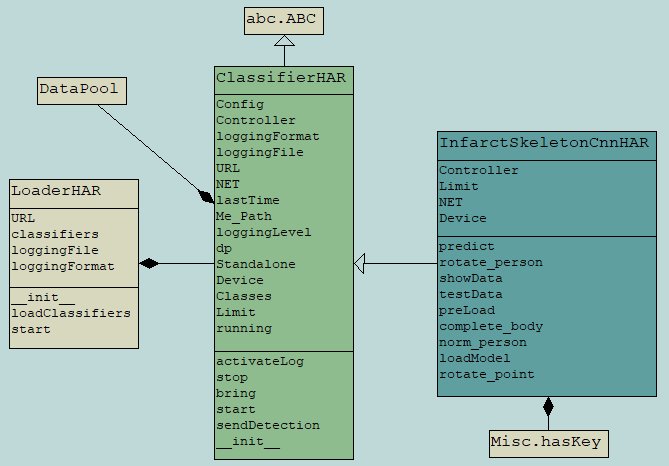
\includegraphics[width=0.9\linewidth]{imgs/04-Construction/04-HarClassModel.PNG}
        	\caption[Modelo de clases de SkeletonInfarctRecognizer]{Modelo de clases de SkeletonInfarctRecognizer. Presenta las la relación y dependencias de las clases del módulo para identificación de eventos de posibles infartos de personas.}
    	    \label{fig:InfarctSkHARClassModel}
        \end{figure}%
        
        El módulo para la identificación de posibles infartos consta de los siguientes archivos:
        
        \begin{itemize}
            \item config.yaml
            \item ColorInfarctRecognizer.py
            \item model/skeletonInfarctModel.h5
        \end{itemize}
        
        El archivo \textbf{config.yaml} contiene las variables mencionadas en la sección \ref{sub2:ConfigFileHAR} donde se resalta especialmente las variables de 'FILTER\_NAME' y 'CLASSES' (ver tabla \ref{Tab:ConfigFileSkeleton}), siendo el tipo de controlador (fuente de información) a filtrar para la inferencia y los eventos a detectar respectivamente.
        
        \begin{table}[ht!]
        \caption[Archivo de configuración de SkeletonInfarctRecognizer]{Atributos del archivo de configuración de ColorInfarctRecognizer.}
        \label{Tab:ConfigFileSkeleton}
        \centering
        \begin{tabular}{ | l p{5cm} p{6cm} | } 
            \hline
            \textbf{Atributo}       & \textbf{Valor} & \textbf{Descripción} \\ 
            \hline\hline
            \textbf{FILTER\_NAME}   & [ 'CamController/rgb', 'CamController/skeleton' ] & de esta forma se consulta las imágenes completas en formato 'RGB' y además los puntos de las articulaciones de las personas detectadas.\\
            \hline
            \textbf{CLASSES}  & [None, Infarct] & Siendo 'None' una clase genérica para indicar la ausencia de evento detectado e 'Infarct' la identificación de una persona con posible infarto.\\
            \hline
            \textbf{MODEL}        & model/SkeletonInfarctModel.h5  &  Entrenamiento previo que permite la identificación de las personas con un posible infarto.\\
            \hline
        \end{tabular}
        \end{table}
        
        El método '\textbf{\textit{predict}}', ejecuta la predicción de si una persona puede estar teniendo un infarto, usando las articulaciones superiores, además extrae el cuadro que contiene el rostro de la persona, para luego pasarlo por las redes que identificaran de forma independiente si la persona tiene una postura equivalente a un infarto, y, además, tiene expresión de dolor (ver alg. \ref{Alg:SkeletonInfarctRecognizerPredict}).
                
        \lstinputlisting[language=Python, caption={Predicción de infarto del módulo SkeletonInfarctRecognizer.}, label=Alg:SkeletonInfarctRecognizerPredict]{code/03-Architecture/SkeletonInfarctRecognizer-predict.py}
\newpage

\section{Construcción del módulo para el reconocimiento de caídas}
\label{Sec:fallDetectModule}
\newpage

\section{Construcción del módulo para envío de alertas}
\label{Sec:AlertModule}
    Esta sección describe la utilización de la plantilla diseñada para la creación de módulos para la notificación de eventos. para ello se seleccionaron dos canales: Correo tradicional y App\index{App} específica con comunicación por Web Sockets (ver \ref{sub:WebSockets}).
    
    \subsection{Módulo para la notificación usando correo electrónico - MailChannel}
    \label{sub:MailChannelComponnent}
        
        Siguiendo los lineamientos de arquitectura se generó el módulo de nombre ``MailChannel'', para la identificación de posibles eventos de infarto.
        
        \begin{figure}[ht!]
        	\centering
        	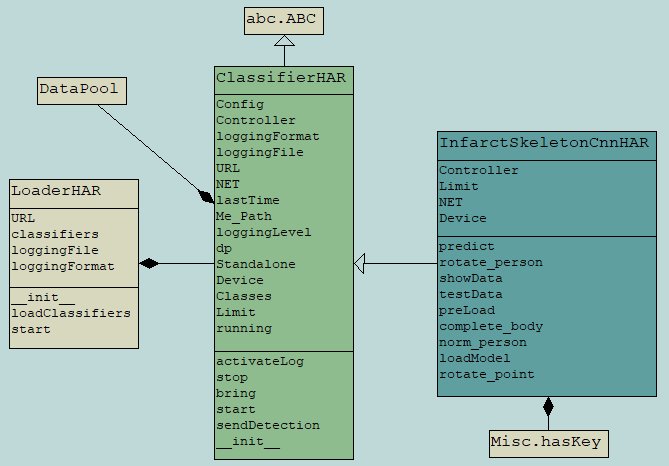
\includegraphics[width=0.9\linewidth]{imgs/04-Construction/04-HarClassModel.PNG}
        	\caption[Modelo de clases de MailChannel]{Modelo de clases de MailChannel. Presenta las la relación y dependencias de las clases del componente que envía alertas a través de correo electrónico.}
    	    \label{fig:MailChannelClassModel}
        \end{figure}%
        
        El componente MailChannel consta de:
        
        \begin{itemize}
            \item config.yaml
            \item MailChannel.py
        \end{itemize}
        
        El archivo \textbf{config.yaml} contiene, además de las variables comunes para todo componente, las mencionadas en la sección \ref{sub2:ConfigFileChannel}.
        
        Por su parte \textbf{MailChannel.py} contiene la lógica específica de envió de correo y dentro de ella, resalta el método '\textbf{trySend}' encargado del envío del mensaje.
\newpage    
    
\section{Construcción del módulo para análisis de eventos complejos}
\label{Sec:AnalyzerModule}

